\documentclass[table]{beamer}
\usepackage[utf8]{inputenc}
\usepackage{amsmath}
\usepackage{upgreek}
\usepackage{graphicx}
\usepackage{verbatim}
\usepackage{subcaption}
\usepackage{amsmath}
\usepackage{hyperref}
\usepackage[export]{adjustbox}
\usepackage{calc}
\usepackage{wrapfig}
\usepackage{xcolor}
\usepackage{tikz}
\definecolor{carolinablue}{rgb}{0.6, 0.73, 0.89}

\usetikzlibrary{shadings, patterns, shapes.geometric}


\newcommand\x{\times}
\newcommand\y{\cellcolor{green!10}}
\usetheme{CambridgeUS}
\title[ACO]{Ant Colony Optimization: A New Meta-heuristic}

\author[Dorigo-Caro]{\ Authors:\\ \ \ \ \ \ Marco Dorigo\ \ \ \ \ \ \ \ \ \   Gianni A. Di Caro\\[4mm]Presented by:\\[2mm]Md. Zawad Abdullah (1605002)\\Bishwajit Bhattacharjee (1605003)\\Md. Mahir Shahriyar (1605024)\\[6mm]Department of CSE,\\Bangladesh University of Engineering and Technology }
\date{\today}

\begin{document}
\maketitle


\begin{frame}{Problem Definition}
	\begin{block}{The Traveling Salesman Problem}
		A salesman needs to visit a number of customers located in different cities and return to the starting city using the shortest route.
	\end{block}
\end{frame}


\begin{frame}{Input:}
	\centering
	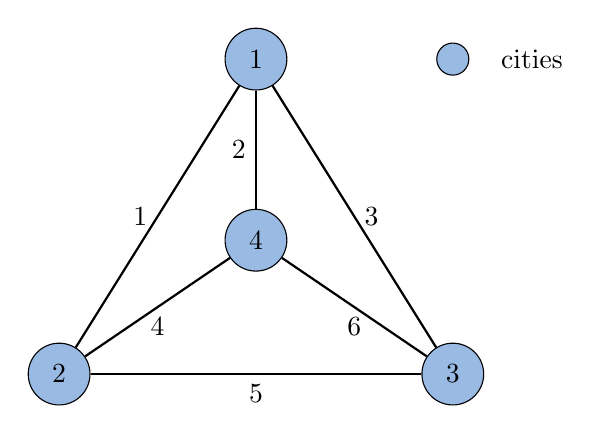
\begin{tikzpicture}
	\node[draw, circle, text width = 0.4cm, align=center, fill = carolinablue] (n2){2};
	\node[draw, circle, xshift = 5cm,text width = 0.4cm, align=center, fill = carolinablue] (n3){3};
	\node[draw, circle, text width = 0.4cm,xshift = 2.5cm,yshift = 4cm, align=center, fill = carolinablue] (n1){1};
	\node[draw, circle, xshift = 2.5cm,yshift = 1.7cm,text width = 0.4cm, align=center, fill = carolinablue] (n4){4};
	\node[draw, circle, xshift = 5cm,yshift = 4cm,text width = 0.1cm, align=center, fill = carolinablue] (n5) {};
	
	\node[draw, rectangle, xshift = .005cm, text width = .8cm, align=center, fill = white, right of = n5, white] (n6) {\textcolor{black}{cities}};
	
	
	\draw[thick] (n1) -- node[left] {1}(n2);
	\draw[thick] (n1) -- node[left] {2}(n4);
	\draw[thick] (n1) -- node[right] {3}(n3);
	
	\draw[thick] (n2) -- node[below] {4}(n4);
	\draw[thick] (n2) -- node[below] {5} (n3);
	
	\draw[thick] (n3) -- node[below] {6} (n4);
	
	%	\draw[->, thick] (cond) -- node[right] {\textcolor{red}{No}} (prob);
	
	\end{tikzpicture}
\end{frame}


\begin{frame}{Output:}
	\centering
	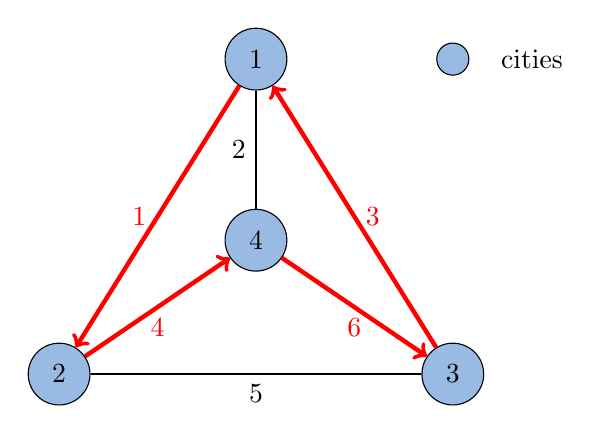
\begin{tikzpicture}
	\node[draw, circle, text width = 0.4cm, align=center, fill = carolinablue] (n2){2};
	\node[draw, circle, xshift = 5cm,text width = 0.4cm, align=center, fill = carolinablue] (n3){3};
	\node[draw, circle, text width = 0.4cm,xshift = 2.5cm,yshift = 4cm, align=center, fill = carolinablue] (n1){1};
	\node[draw, circle, xshift = 2.5cm,yshift = 1.7cm,text width = 0.4cm, align=center, fill = carolinablue] (n4){4};
	\node[draw, circle, xshift = 5cm,yshift = 4cm,text width = 0.1cm, align=center, fill = carolinablue] (n5) {};
	
	\node[draw, rectangle, xshift = .005cm, text width = .8cm, align=center, fill = white, right of = n5, white] (n6) {\textcolor{black}{cities}};
	
	
	\draw[ultra thick,red,->] (n1) -- node[left] {1}(n2);
	\draw[thick] (n1) -- node[left] {2}(n4);
	\draw[ultra thick,red,<-] (n1) -- node[right] {3}(n3);
	
	\draw[ultra thick,red,->] (n2) -- node[below] {4}(n4);
	\draw[thick] (n2) -- node[below] {5} (n3);
	
	\draw[ultra thick,red,<-] (n3) -- node[below] {6} (n4);
	
	%	\draw[->, thick] (cond) -- node[right] {\textcolor{red}{No}} (prob);
	
	\end{tikzpicture}
\end{frame}

\begin{frame}{Known Methods}

	\begin{itemize}
		\item <1->	Backtracking\\
					\uncover<2->{Issue - Complexity is exponential.}\\
					\uncover<3->{\textbf{Not Good Enough!}}
		\vspace{\baselineskip}	\vspace{\baselineskip}
		\uncover<4->{\item <2->	Bitmask DP\\}
					\uncover<5->{Issue - Works efficiently when input is small.}\\
					\uncover<6->{\textbf{Not Good Enough!}}
	\end{itemize}
\end{frame}


\begin{frame}{Motivation}
	\centering
	\textbf{We will use Ant Colony Optimization (ACO) to solve TSP more efficiently.}
\end{frame}


\begin{frame}{Ants collecting food-1}
	\begin{figure}
		\centering
		\def\svgscale{0.6}
		\input{AntSearch.pdf_tex}
	\end{figure}
	\ \ \ \ \ \ \ \ \ \ \ \ \ \ \ \ \ \ \ \ {\color{blue}Figure:} Paths From Food to Ants' Nest
\end{frame}

\begin{frame}{Ants collecting food-2}
		\begin{figure}
			\centering
			\def\svgscale{0.6}
			\input{AntSearch2.pdf_tex}
		\end{figure}
		\ \ \ \ \ \ \ \ \ \ \ \ \ \ \ \ \ \ \ \ \ \ \ \ \ {\color{blue}Figure:} Ants Searching for Food
\end{frame}


\begin{frame}{Ants collecting food-3}
		\begin{figure}
			\centering
			\def\svgscale{0.6}
			\input{AntSearch3.pdf_tex}
		\end{figure}
		\ \ \ \ \ \ \ \ \ \ \ \ \ \ \ \ \ \ \ \ \ \ \ \ \ {\color{blue}Figure:} Ants Following An Optimal Path
\end{frame}


\begin{frame}
	\centering
	\vspace{\baselineskip}	\vspace{\baselineskip}
	So how do they communicate??\\ 
	{\vspace{\baselineskip}	\vspace{\baselineskip}}
	\uncover<2->{\textcolor{red}{\huge Pheromone}}
	\vspace{\baselineskip}	\vspace{\baselineskip}
	\begin{figure}
		\uncover<3>{\includegraphics[ width=.7\textwidth,left ]{AntPheromone.png}	}
	\end{figure}
\end{frame}

\begin{frame}
	\centering
	\vspace{\baselineskip}	\vspace{\baselineskip}
	So how do they communicate??\\ 
	{\vspace{\baselineskip}	\vspace{\baselineskip}}
	{\textcolor{red}{\huge Pheromone}}
	\vspace{\baselineskip}	\vspace{\baselineskip}
	\begin{figure}
		{\includegraphics[ width=1\textwidth,right ]{AntPheromone3.png}	}
	\end{figure}
\end{frame}


\begin{frame}
	\centering
	\vspace{\baselineskip}	\vspace{\baselineskip}
	So how do they communicate??\\ 
	{\vspace{\baselineskip}	\vspace{\baselineskip}}
	{\textcolor{red}{\huge Pheromone}}
	\vspace{\baselineskip}	\vspace{\baselineskip}
	\begin{figure}
		{\includegraphics[ width=1\textwidth,right ]{AntPheromone2.png}	}
	\end{figure}
\end{frame}


\begin{frame}
	\centering
	\vspace{\baselineskip}	\vspace{\baselineskip}
	So how do they communicate??\\ 
	{\vspace{\baselineskip}	\vspace{\baselineskip}}
	{\textcolor{red}{\huge Pheromone}}
	\vspace{\baselineskip}	\vspace{\baselineskip}
	\begin{figure}
		{\includegraphics[ width=1\textwidth,right ]{AntPheromone3.png}	}
	\end{figure}
\end{frame}





\begin{frame}{Previous Works}
	\begin{columns}
	   	\column{0.5\textwidth}
		\begin{itemize}
			\item In the year 1991, Marco Dorigo proposed an algorithm called "Ant System".
			
			\vspace{\baselineskip}	\vspace{\baselineskip}
			
			\item  AS was first applied to the Traveling Salesman Problem.
			
			
		\end{itemize}
	   	\column{0.5\textwidth}
			\begin{figure}[h]
				\centering
				\includegraphics[width=0.7\textwidth]{Dorigo.jpg}
				\caption{Marco Dorigo}
			\end{figure}
	\end{columns}

	
	
\end{frame}

\begin{frame}{Results}
	\centering
	A more efficient algorithm to solve TSP is the ACO meta-heuristic.
\end{frame}

\section{Methods}
\begin{frame}{Notations}
	
	\begin{columns}
		\begin{column}{0.5\textwidth}
			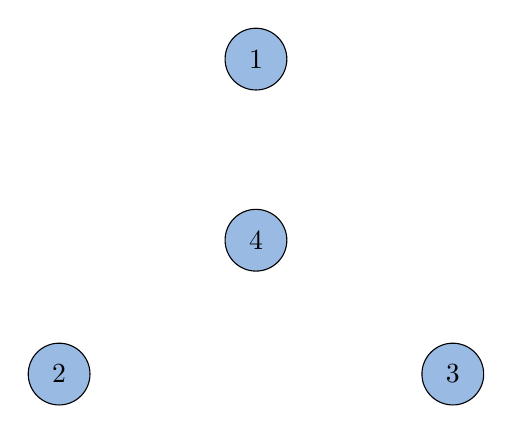
\begin{tikzpicture}
			\node[draw, circle, text width = 0.4cm, align=center, fill = carolinablue] (n2){2};
			\node[draw, circle, xshift = 5cm,text width = 0.4cm, align=center, fill = carolinablue] (n3){3};
			\node[draw, circle, text width = 0.4cm,xshift = 2.5cm,yshift = 4cm, align=center, fill = carolinablue] (n1){1};
			\node[draw, circle, xshift = 2.5cm,yshift = 1.7cm,text width = 0.4cm, align=center, fill = carolinablue] (n4){4};
			
			
			\end{tikzpicture}
		\end{column}
		
		\begin{column}{0.5\textwidth}
			$ C = \{c_1,c_2,...,c_{N_C} \} $ is the set of \textit{cities}.
		\end{column}
	\end{columns}
	
\end{frame}


\begin{frame}{Notations Continued..}
	
	\begin{columns}
		\begin{column}{0.5\textwidth}
			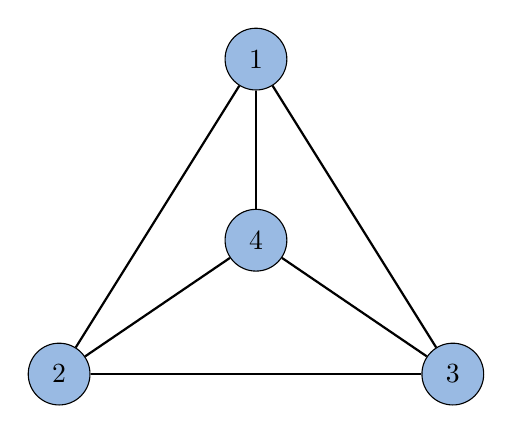
\begin{tikzpicture}
			\node[draw, circle, text width = 0.4cm, align=center, fill = carolinablue] (n2){2};
			\node[draw, circle, xshift = 5cm,text width = 0.4cm, align=center, fill = carolinablue] (n3){3};
			\node[draw, circle, text width = 0.4cm,xshift = 2.5cm,yshift = 4cm, align=center, fill = carolinablue] (n1){1};
			\node[draw, circle, xshift = 2.5cm,yshift = 1.7cm,text width = 0.4cm, align=center, fill = carolinablue] (n4){4};
			
			\draw[thick] (n1) -- (n2);
			\draw[thick] (n1) -- (n4);
			\draw[thick] (n1) -- (n3);
			
			\draw[thick] (n2) -- (n4);
			\draw[thick] (n2) -- (n3);
			
			\draw[thick] (n3) -- (n4);
			
			\end{tikzpicture}
		\end{column}
		
		\begin{column}{0.5\textwidth}
			$ L = \{l_{c_{i}c_{j}}\ |\ (c_i,c_j)\ \in  \tilde{C}\},\ |L| \leq N^{2}_C $ is the set of \textit{connections} between \textit{cities}.
		\end{column}
	\end{columns}
	
\end{frame}



\begin{frame}{Notations Continued..}
	\begin{columns}
		\begin{column}{0.5\textwidth}
			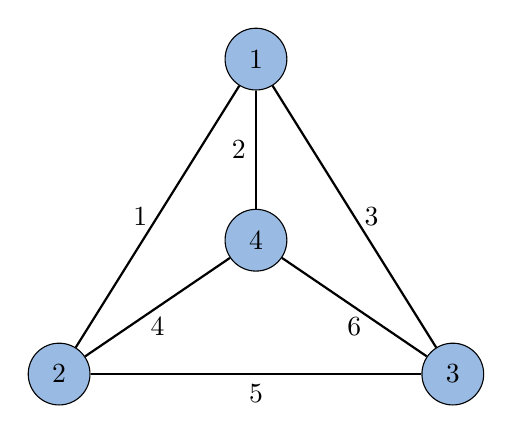
\begin{tikzpicture}
			\node[draw, circle, text width = 0.4cm, align=center, fill = carolinablue] (n2){2};
			\node[draw, circle, xshift = 5cm,text width = 0.4cm, align=center, fill = carolinablue] (n3){3};
			\node[draw, circle, text width = 0.4cm,xshift = 2.5cm,yshift = 4cm, align=center, fill = carolinablue] (n1){1};
			\node[draw, circle, xshift = 2.5cm,yshift = 1.7cm,text width = 0.4cm, align=center, fill = carolinablue] (n4){4};
			
			\draw[thick] (n1) -- node[left] {1}(n2);
			\draw[thick] (n1) -- node[left] {2}(n4);
			\draw[thick] (n1) -- node[right] {3}(n3);
			
			\draw[thick] (n2) -- node[below] {4}(n4);
			\draw[thick] (n2) -- node[below] {5} (n3);
			
			\draw[thick] (n3) -- node[below] {6} (n4);
			
			%	\draw[->, thick] (cond) -- node[right] {\textcolor{red}{No}} (prob);
			
			\end{tikzpicture}
		\end{column}
		
		\begin{column}{0.5\textwidth}
			$ J_{c_ic_j} \equiv J(l_{c_ic_j}) $ is a \emph{cost} function associated with each \textit{connection} $l_{c_ic_j} \in L $.
		\end{column}
	\end{columns}
	
\end{frame}


\begin{frame}{Notations Continued..}
	\begin{columns}
		\begin{column}{0.5\textwidth}
			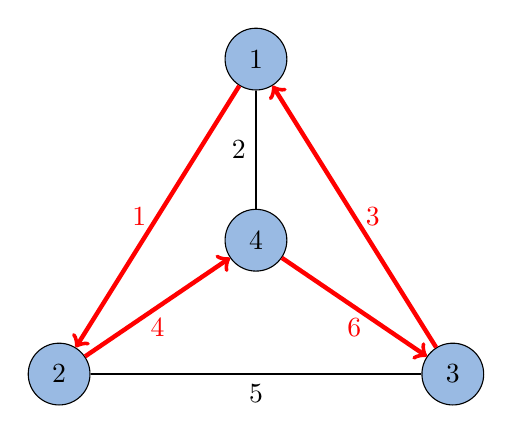
\begin{tikzpicture}
			\node[draw, circle, text width = 0.4cm, align=center, fill = carolinablue] (n2){2};
			\node[draw, circle, xshift = 5cm,text width = 0.4cm, align=center, fill = carolinablue] (n3){3};
			\node[draw, circle, text width = 0.4cm,xshift = 2.5cm,yshift = 4cm, align=center, fill = carolinablue] (n1){1};
			\node[draw, circle, xshift = 2.5cm,yshift = 1.7cm,text width = 0.4cm, align=center, fill = carolinablue] (n4){4};
			
			\draw[ultra thick,red,->] (n1) -- node[left] {1}(n2);
			\draw[thick] (n1) -- node[left] {2}(n4);
			\draw[ultra thick,red,<-] (n1) -- node[right] {3}(n3);
			
			\draw[ultra thick,red,->] (n2) -- node[below] {4}(n4);
			\draw[thick] (n2) -- node[below] {5} (n3);
			
			\draw[ultra thick,red,<-] (n3) -- node[below] {6} (n4);
			
			%	\draw[->, thick] (cond) -- node[right] {\textcolor{red}{No}} (prob);
			
			\end{tikzpicture}
		\end{column}
		
		\begin{column}{0.5\textwidth}
			$ J_{\psi}(L) $ is the \emph{cost function} associated to each solution 	$\psi $. It is the summation of all the costs $ J(c_i,c_j) $ of all the connections belonging to the solution $\psi $ .
		\end{column}
	\end{columns}
	\vspace{\baselineskip} 	\vspace{\baselineskip}
	\centering
	\textcolor{red}{\centering The optimal cost here is $1 + 4 + 6 + 3 = 14 $ }
	
\end{frame}

\begin{frame}{Ant Properties}
	
	\begin{columns}
		
		
		\begin{column}{0.4\textwidth}
			\begin{itemize}
				\item	Every ant has its own memory.
			\end{itemize}
		\end{column}
		
		\begin{column}{0.6\textwidth}
			\begin{figure}
				\centering
				\includegraphics[width=\textwidth ]{AntWithMemory.png}
			\end{figure}
		\end{column}
	\end{columns}
\end{frame}	



\begin{frame}{Ant Properties Continued}
	
	\begin{columns}
		
		
		\begin{column}{0.4\textwidth}
			\begin{itemize}
				\item	An ant chooses the next node to visit from its memory and the ant-routing table
			\end{itemize}
		\end{column}
		
		\begin{column}{0.6\textwidth}
			\begin{figure}
				\centering
				\includegraphics[width=\textwidth ]{WhereToGo.png}
			\end{figure}
		\end{column}
	\end{columns}
\end{frame}	

\begin{frame}{Ant Properties Continued}	
	\begin{columns}
		
		\begin{column}{0.6\textwidth}
			\resizebox{\linewidth}{!}{$
				\label{eq:appendrow}
				\left(\begin{array}{cccc}
				0  & 5  & 3 & 1 \\
				4   & 0  & 1 & 6 \\
				9   & 3   & 0 & 9 \\
				12   & 4   & 15  & 0 \\
				\end{array}\right)
				$}
		
		\centering
		\vspace{\baselineskip}
		\Large Ant-routing table, $ \mathnormal{a} $
		\end{column}
		\begin{column}{0.4\textwidth}
			\centering
			Here, $ \mathnormal{a_{ij}} $ is a measurement of the quality of the edge from node $i$ to node $j$.
		\end{column}
	\end{columns}
\end{frame}

\begin{frame}{Formula for ant-routing table}

	The formula for updating the ant-routing table is:
	
	{\Large $$
		\Large a_{ij} = \frac { {[\uptau_{ij}(t)]}^{\alpha} {[\eta_{ij}]}^{\beta} }
		{\displaystyle\sum_{l \in \mathcal{N}_i} {[\uptau_{il}(t)]}^{\alpha} {[\eta_{il}]}^{\beta} } 
		\ \ \ \ \ \ \ \forall j \in \mathcal{N}_i
		$$}
	
	\begin{itemize}
		\item  $ {\uptau_{ij}} $ is the intensity of pheromone trail of the  edge $ 	\mathnormal{l_{ij}} $
		
		\item $ {\eta_{ij}} $ is the heuristic value of the edge between $i$ and $j$.	
		{\Large $$ {\eta_{ij}} = \frac{1}{J_{c_ic_j}} $$ }
		
		\item $\alpha$ and $\beta$ are two parameters that control the relative weight of pheromone trail and heuristic value. 
	\end{itemize}
	
\end{frame}

\begin{frame}{Formula for ant-routing table Continued}
	The probability $\mathnormal{p}^{k}_{ij}(t)$ with which an ant $k$ located in city $i$ chooses the city $ j \in \mathcal{N}_i^k $ to move to at the $t$-th  iteration is: 
	
	{\Large 
		$$ \mathnormal{p}^{k}_{ij}(t) = \frac{ {a}_{ij}(t) } 
		{ \displaystyle\sum_{l \in \mathcal{N}_{i}^{k}} a_{il}(t) }
		$$}
	
	where $\mathcal{N}_i^k \subseteq \mathcal{N}_i $ is the feasible neighborhood of node $i$ for ant $k$.
	
\end{frame}


\begin{frame}{Pheromone Trail Evaporation}
	After pheromone updating has been performed by the ants, pheromone evaporation is triggered: the following rule is applied to all the edges $l_{ij}$ of the graph $G$
	
	{\Large
		$$
		\uptau_{ij}(t) \leftarrow (1-\rho)\uptau_{ij}(t)
		$$}\newline
	where $ \rho \in (0,1] $ is the pheromone trail decay coefficient.
\end{frame}


\begin{frame}{\textbf{procedure} ACO\_meta-heuristic()}
	\centering
	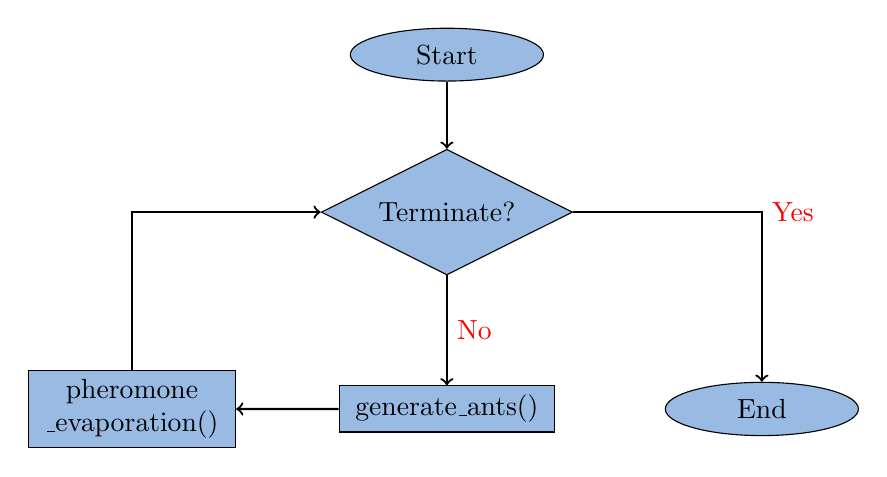
\begin{tikzpicture}
	\node[draw, ellipse, text width = 1.5cm, align=center, yshift=-2cm, fill = carolinablue] (start){Start};
	
	\node[draw, diamond, align=center, below of= start, , text width = 2cm, yshift = -1cm, aspect=2, fill = carolinablue] (cond){Terminate?};
	
	\node[draw, rectangle, align=center, below of= cond, , text width = 2.5cm, yshift = -1.5cm, fill = carolinablue] (activity){generate\_ants()};
	
	\node[draw, rectangle, align=center, left  of= cond, , text width = 2.4cm, xshift = -3cm, yshift=-2.5cm, fill = carolinablue] (eva){pheromone\\\_evaporation()};
	
	\node[draw, ellipse, right of = activity, text width = 1.5cm, xshift = 3cm, align=center, fill = carolinablue] (end){End};
	
	\draw[->, thick] (start) -- (cond);
	
	\draw[->, thick] (cond) -- node[right] {\textcolor{red}{No}} (activity);
	
	\draw[->, thick] (activity) -- (eva);
	
	\draw[->, thick] (eva) |- (cond);
	
	\draw[->, thick] (cond) -| node[right] {\textcolor{red}{Yes}} (end);
	\end{tikzpicture}
\end{frame}

\begin{frame}{\textbf{procedure} generate\_ants()}
	\centering
	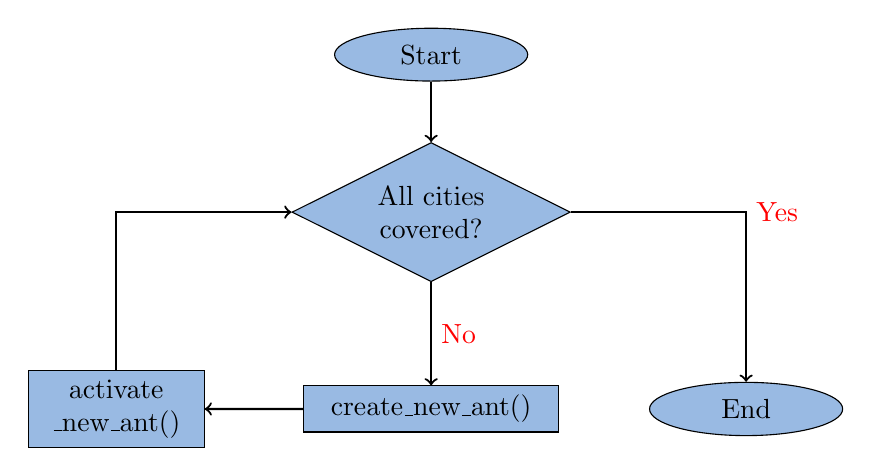
\begin{tikzpicture}
	\node[draw, ellipse, text width = 1.5cm, align=center, yshift=-2cm, fill = carolinablue] (start){Start};
	
	\node[draw, diamond, align=center, below of= start, , text width = 1.5cm, yshift = -1cm, aspect=2, fill = carolinablue] (cond){All cities\\covered?};
	
	\node[draw, rectangle, align=center, below of= cond, , text width = 3cm, yshift = -1.5cm, fill = carolinablue] (creation){create\_new\_ant()};
	
	\node[draw, rectangle, align=center, left  of= cond, text width = 2cm, xshift = -3cm, yshift=-2.5cm, fill = carolinablue] (eva){activate\\\_new\_ant()};
	
	\node[draw, ellipse, right of = creation, text width = 1.5cm, xshift = 3cm, align=center, fill = carolinablue] (end){End};
	
	\draw[->, thick] (start) -- (cond);
	
	\draw[->, thick] (cond) -- node[right] {\textcolor{red}{No}} (creation);
	
	\draw[->, thick] (creation) -- (eva);
	
	\draw[->, thick] (eva) |- (cond);
	
	\draw[->, thick] (cond) -| node[right] {\textcolor{red}{Yes}} (end);
	\end{tikzpicture}
\end{frame}

\begin{frame}{\textbf{procedure} activate\_new\_ant() \{Ant lifecycle\}}
	
	\centering
	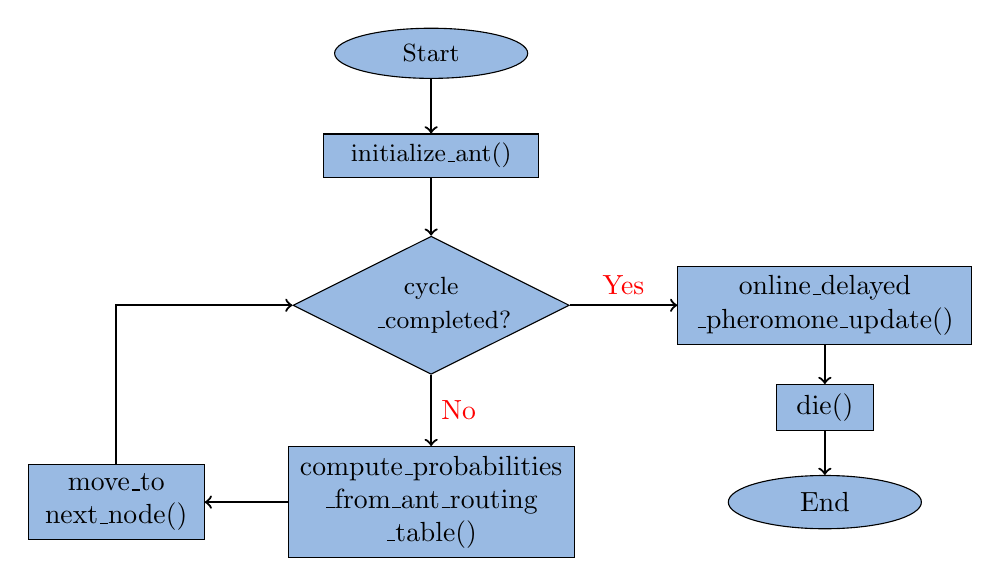
\begin{tikzpicture}
	\node[draw, ellipse, text width = 1.5cm, align=center, fill = carolinablue] (start){\small Start};
	
	\node[draw, rectangle, align=center, below of= start, text width = 2.5cm, yshift = -.3cm, fill = carolinablue] (initialize){\small initialize\_ant()};
	
	\node[draw, diamond, align=center, below of= initialize, text width = 1.4cm, yshift = -.9cm, aspect=2, fill = carolinablue] (cond){\small cycle\\\_completed?};
	
	\node[draw, rectangle, align=center, right of= cond, text width = 3.5cm, xshift=4cm, fill = carolinablue] (update){online\_delayed\\\_pheromone\_update()};
	
	\node[draw, rectangle, align=center, below of= cond, , text width = 3.4cm, yshift = -1.5cm, fill = carolinablue] (prob){compute\_probabilities\\\_from\_ant\_routing\\\_table()};
	
	\node[draw, ellipse, right of = prob, text width = 1.5cm, xshift = 4cm, align=center, fill = carolinablue] (end){End};
	
	\node[draw, rectangle, align=center, above of= end, text width = 1cm, yshift=.2cm, fill = carolinablue] (die){die()};
	
	\node[draw, rectangle, align=center, left  of= prob, text width = 2cm, xshift = -3cm, fill = carolinablue] (move){move\_to\\next\_node()};
	
	\draw[->, thick] (start) -- (initialize);
	
	\draw[->, thick] (initialize) -- (cond);
	
	\draw[->, thick] (cond) -- node[right] {\textcolor{red}{No}} (prob);
	
	\draw[->, thick] (prob) -- (move);
	
	\draw[->, thick] (move) |- (cond);
	
	\draw[->, thick] (cond) -- node[above] {\textcolor{red}{Yes}} (update);
	
	\draw[->, thick] (update) -- (die);
	
	\draw[->, thick] (die) -- (end);
	\end{tikzpicture}
\end{frame}



\begin{frame}{Conclusions}
	\centering
	\large ACO is a new weapon to attack NP-hard graph problem!!\\
\end{frame}
\end{document}